\section{Volume by The Shell Method} \label{S:6.2.ShellMethod}

\begin{goals}
\item Is there other methods to use a definite integral to find the volume of a three-dimensional solid  or a solid of revolution that results from revolving a two-dimensional region about a particular axis? 
\item In what circumstances do we integrate with respect to $y$ instead of integrating with respect to $x$?
\item When is it better to use the Shell Method as oppossed to the Washer Method? 
\end{goals}

%-------------------------------
% SUBSECTION INTRODUCTION
%-------------------------------
\subsection*{Introduction}

Often a given problem can be solved in more than one way. A particular method may be chosen out of convenience, personal preference, or perhaps necessity. Ultimately, it is good to have options.

The previous section introduced the Disk and Washer Methods, which computed the volume of solids of revolution by integrating the cross-sectional area of the solid. This section develops another method of computing volume, the \textbf{Shell Method.} Instead of slicing the solid perpendicular to the axis of rotation creating cross-sections, we now slice it parallel to the axis of rotation, creating ``shells.''

The Preview Activity \ref{PA:6.2} introduces a situation where using the Washer Method from Section \ref{S:6.1.Volume} becomes very tedious. 

\begin{marginfigure}[8cm] % MARGIN FIGURE
\margingraphics{figs/6/PA62.pdf}
\caption{The circular cone described in Preview Activity~\ref{PA:6.2}} \label{F:PA.6.2}
\end{marginfigure}

\begin{pa} \label{PA:6.2}  Consider the function $f(x)=x^2-x^3$, whose graph is in Figure~\ref{F:PA.6.2}.  Our goal in this activity is to use a definite integral to determine the volume of the solid formed by revolving the region bounded by $f(x)$ and $y=0$ about the $y$-axis.

\ba
\item Using the Washer Method, find an expression for the inner and outer radii of a slice.
\item Set up a definite integral to find the volume. If you try to evaluate the integral, what do you notice that happens? 
\item Find where the local maximum occurs.  
\item Use the results of past c) to split the solid into two pieces. Set up two definite integrals to find the volume of the original solid.  
	
\ea
\end{pa} 
\afterpa % PREVIEW need use f=x^2-x^3 and have do disk method

Consider Figure~\ref{fig:6.2.shell}-(a), where the region shown rotated around the $y$-axis forming the solid shown in Figure~\ref{fig:6.2.shell}-(b). A small slice of the region is drawn in Figure~\ref{fig:6.2.shell}-(a), parallel to the axis of rotation. When the region is rotated, this thin slice forms a \textbf{cylindrical shell}, as pictured in Figure~\ref{fig:6.2.shell}-(c). The previous section approximated a solid with lots of thin disks (or washers); we now approximate a solid with many thin cylindrical shells. 

To compute the volume of one shell, first consider the paper label on a soup can with radius $r$ and height $h$. What is the area of this label? A simple way of determining this is to cut the label and lay it out flat, forming a rectangle with height $h$ and length $2\pi r$. Thus the area is $A = 2\pi rh$; see Figure~\ref{F:6.2.soupcan}-(a).

\begin{marginfigure}[-1cm] % MARGIN FIGURE
\begin{center}
\subfloat[]{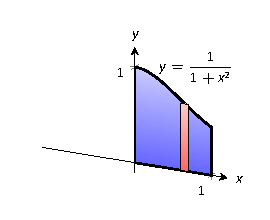
\includegraphics[scale=.95]{figures/figshell_intro_b}}

\subfloat[]{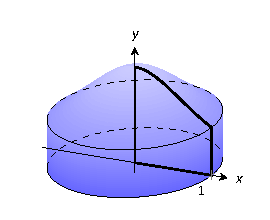
\includegraphics[scale=.95]{figures/figshell_intro_a}}

\subfloat[]{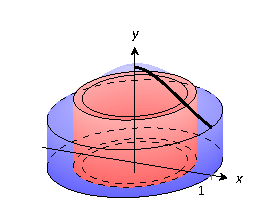
\includegraphics[scale=.95]{figures/figshell_intro_d}}
\caption{Introducing the Shell Method.}\label{fig:6.2.shell}
\end{center}
\end{marginfigure}

Do a similar process with a cylindrical shell, with height $h$, thickness $\Delta x$, and approximate radius $r$. Cutting the shell and laying it flat forms a rectangular solid with length $2\pi r$, height $h$ and depth $\dx$. Thus the volume is $V \approx 2\pi rh\dx$; see Figure~\ref{F:6.2.soupcan}-(b). (We say ``approximately'' since our radius was an approximation.)

By breaking the solid into $n$ cylindrical shells, we can approximate the volume of the solid as
$$V = \sum_{i=1}^n 2\pi r_ih_i\dx_i,$$ where $r_i$, $h_i$ and $\dx_i$ are the radius, height and thickness of the $i\,^\text{th}$ shell, respectively. 

This is a Riemann Sum. Taking a limit as the thickness of the shells approaches $0$ leads to a definite integral.

\begin{marginfigure}[1cm] % MARGIN FIGURE
\subfloat[]{\margingraphics{figures/figshell_soupcan}}

\subfloat[]{\margingraphics{figures/figshell_unwrapshell}}
\caption{Determining the volume of a thin cylindrical shell.}\label{F:6.2.soupcan}
\end{marginfigure}

\concept{The Shell Method} % CONCEPT
{Let a solid be formed by revolving a region $R$, bounded by $x=a$ and $x=b$, around a vertical axis. Let $r(x)$ represent the distance from the axis of rotation to $x$ (i.e., the radius of a sample shell) and let $h(x)$ represent the height of the solid at $x$ (i.e., the height of the shell). The volume of the solid is 
\index{integration!volume!Shell Method}\index{Shell Method}
$$V = 2\pi\int_a^b r(x)h(x)\ dx.$$
} %end CONCEPT

\textbf{Special Cases:}
\begin{enumerate}[1)]
\item When the region $R$ is bounded above by $y=f(x)$ and below by $y=g(x)$, then $h(x) = f(x)-g(x)$.
\item	When the axis of rotation is the $y$-axis (i.e., $x=0$) then $r(x) = x$.
\end{enumerate}
	
Let's practice using the Shell Method.

\begin{example} \label{eg:6.2.1} % EXAMPLE
Find the volume of the solid formed by rotating the region bounded by $y=0$, $y=1/(1+x^2)$, $x=0$ and $x=1$ about the $y$-axis.

\solution This is the region used to introduce the Shell Method in Figure~\ref{fig:6.2.shell}, but is sketched again in Figure~\ref{F:6.2.Ex1} for closer reference. A line is drawn in the region parallel to the axis of rotation representing a shell that will be carved out as the region is rotated about the $y$-axis. (This is the differential element.)

The distance this line is from the axis of rotation determines $r(x)$; as the distance from $x$ to the $y$-axis is $x$, we have $r(x)=x$. The height of this line determines $h(x)$; the top of the line is at $y=1/(1+x^2)$, whereas the bottom of the line is at $y=0$. Thus $h(x) = 1/(1+x^2)-0 = 1/(1+x^2)$. The region is bounded from $x=0$ to $x=1$, so the volume is 
\begin{align*}
V 	&= 2\pi\int_0^1 \frac{x}{1+x^2}\ dx. \\
\intertext{This requires substitution. Let $u=1+x^2$, so $du = 2x\ dx$. We also change the bounds: $u(0) = 1$ and $u(1) = 2$. Thus we have:}
&= \pi\int_1^2 \frac{1}{u}\ du \\
&= \pi\ln u\Big|_1^2\\
&= \pi\ln 2 \approx 2.178 \ \text{units}^3.
\end{align*}
Note: in order to find this volume using the Disk Method, two integrals would be needed to account for the regions above and below $y=1/2$.
\end{example}

\begin{marginfigure}[-14cm] %MARGIN FIGURE
\margingraphics{figures/figshell1}
\caption{Graphing a region in Example~\ref{eg:6.2.1}.} \label{F:6.2.Ex1}
\end{marginfigure} % EXAMPLE

With the Shell Method, nothing special needs to be accounted for to compute the volume of a solid that has a hole in the middle, as demonstrated next.

\begin{marginfigure}[2cm] %MARGIN FIGURE
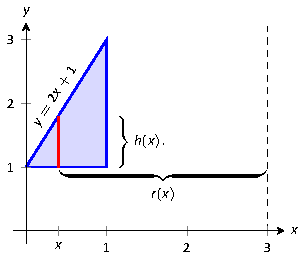
\includegraphics{figures/figshell2a}
\caption{Graphing a region in Example~\ref{eg:6.2.2}.} \label{F:6.2.Ex2a}
\end{marginfigure}

\begin{example} \label{eg:6.2.2} % EXAMPLE
Find the volume of the solid formed by rotating the triangular region determined by the points $(0,1)$, $(1,1)$ and $(1,3)$ about the line $x=3$.

\solution
The region is sketched in Figure \ref{F:6.2.Ex2a} along with the differential element, a line within the region parallel to the axis of rotation. 

The height of the differential element is the distance from $y=1$ to $y=2x+1$, the line that connects the points $(0,1)$ and $(1,3)$. Thus $h(x) = 2x+1-1 = 2x$. The radius of the shell formed by the differential element is the distance from $x$ to $x=3$; that is, it is $r(x)=3-x$. The $x$-bounds of the region are $x=0$ to $x=1$, giving
\begin{align*}
V &=	2\pi\int_0^1 (3-x)(2x)\ dx \\
	&= 2\pi\int_0^1 \big(6x-2x^2)\ dx \\
	&= 2\pi\left(3x^2-\frac23x^3\right)\Big|_0^1\\
	&= \frac{14}{3}\pi\approx 14.66 \ \text{units}^3.
\end{align*}
\end{example}

\begin{marginfigure}[-5cm] %MARGIN FIGURE
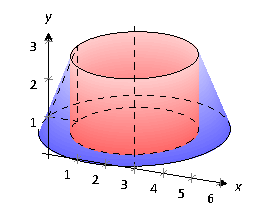
\includegraphics{figures/figshell2b}
\caption{Graphing a region in Example~\ref{eg:6.2.2}.} \label{F:6.2.Ex2b}
\end{marginfigure} % EXAMPLE

\begin{activity} \label{A:6.2.1}  
In each of the following questions, draw a careful, labeled sketch of the region described, as well as the resulting solid that results from revolving the region about the stated axis.  In addition, draw a representative slice and state the volume of that slice, along with a definite integral whose value is the volume of the entire solid.  It is not necessary to evaluate the integrals you find.
\ba
	\item The region $S$ bounded by the $y$-axis, the curve $y = \sqrt{x}$, and the line $y = 2$; revolve $S$ about the $y$-axis.
	\item The region $S$ bounded by the $x$-axis, the curve $y = \sqrt{x}$, and the line $x = 4$; revolve $S$ about the $y$-axis.
	\item The finite region $S$ in the first quadrant bounded by the curves $y = 2x$ and $y = x^3$; revolve $S$ about the $y$-axis.
	\item The finite region $S$ bounded by the curves $x = (y-1)^2$ and $y  = x-1$; revolve $S$ about the $y$-axis.
	\item How do you answers to this activity compare to the results of Activty \ref{A:6.1.2}?
\ea

\end{activity}
\begin{smallhint}
\ba
	\item Small hints for each of the prompts above.
\ea
\end{smallhint}
\begin{bighint}
\ba
	\item Big hints for each of the prompts above.
\ea
\end{bighint}
\begin{activitySolution}
\ba
	\item Solutions for each of the prompts above.
\ea
\end{activitySolution}
\aftera
 % ACTIVITY

When revolving a region around a horizontal axis, we must consider the radius and height functions in terms of $y$, not $x$.

\begin{marginfigure}[6cm] %MARGIN FIGURE
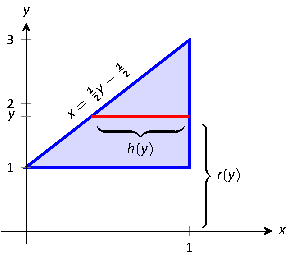
\includegraphics{figures/figshell3a}
\caption{Graphing a region in Example~\ref{eg:6.2.3}.} \label{F:6.2.Ex3a}
\end{marginfigure}

\begin{example} \label{eg:6.2.3} % EXAMPLE
Find the volume of the solid formed by rotating the region given in Example~\ref{eg:6.2.2} about the $x$-axis.

\solution
The region is sketched in Figure~\ref{F:6.2.Ex3a} with a sample differential element and the solid is sketched in Figure~\ref{F:6.2.Ex3b}. (Note that the region looks slightly different than it did in the previous example as the bounds on the graph have changed.)

The height of the differential element is an $x$-distance, between $x=\frac12y-\frac12$ and $x=1$. Thus $h(y) = 1-(\frac12y-\frac12) = -\frac12y+\frac32.$ The radius is the distance from $y$ to the $x$-axis, so $r(y) =y$. The $y$ bounds of the region are $y=1$ and $y=3$, leading to the integral

\begin{align*}
V &= 2\pi\int_1^3\left[y\left(-\frac12y+\frac32\right)\right]\ dy \\
	&= 2\pi\int_1^3\left[-\frac12y^2+\frac32y\right]\ dy \\
	&= 2\pi\left[-\frac16y^3+\frac34y^2\right]\Big|_1^3 \\
	&= 2\pi\left[\frac94-\frac7{12}\right]\\
	&=	\frac{10}{3}\pi \approx 10.472\ \text{units}^3.
\end{align*}
\end{example}

\begin{marginfigure}[-6cm] %MARGIN FIGURE
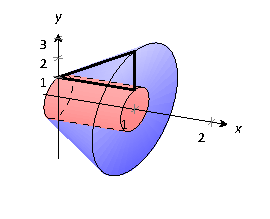
\includegraphics{figures/figshell3b}
\caption{Graphing a region in Example~\ref{eg:6.2.3}.} \label{F:6.2.Ex3b}
\end{marginfigure} % EXAMPLE

\begin{activity} \label{A:6.2.2}  
In each of the following questions, draw a careful, labeled sketch of the region described, as well as the resulting solid that results from revolving the region about the stated axis.  In addition, draw a representative slice and state the volume of that slice, along with a definite integral whose value is the volume of the entire solid.  It is not necessary to evaluate the integrals you find.
\ba
	\item The region $S$ bounded by the $y$-axis, the curve $y = \sqrt{x}$, and the line $y = 2$; revolve $S$ about the $y$-axis.
	\item The region $S$ bounded by the $x$-axis, the curve $y = \sqrt{x}$, and the line $x = 4$; revolve $S$ about the $y$-axis.
	\item The finite region $S$ in the first quadrant bounded by the curves $y = 2x$ and $y = x^3$; revolve $S$ about the $x$-axis.	
	\item The finite region $S$ in the first quadrant bounded by the curves $y = 2x$ and $y = x^3$; revolve $S$ about the $y$-axis.
	\item The finite region $S$ bounded by the curves $x = (y-1)^2$ and $y  = x-1$; revolve $S$ about the $y$-axis
\ea

\end{activity}
\begin{smallhint}
\ba
	\item Small hints for each of the prompts above.
\ea
\end{smallhint}
\begin{bighint}
\ba
	\item Big hints for each of the prompts above.
\ea
\end{bighint}
\begin{activitySolution}
\ba
	\item Solutions for each of the prompts above.
\ea
\end{activitySolution}
\aftera
 % ACTIVITY

At the beginning of this section it was stated that ``it is good to have options.'' The next example finds the volume of a solid rather easily with the Shell Method, but using the Washer Method would be quite a chore.

\begin{marginfigure}[7cm] %MARGIN FIGURE
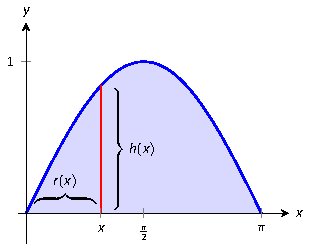
\includegraphics{figures/figshell4a}
\caption{Graphing a region in Example~\ref{eg:6.2.4}.} \label{F:6.2.Ex4a}
\end{marginfigure}

\begin{example} \label{eg:6.2.4} % EXAMPLE
Find the volume of the solid formed by revolving the region bounded by $y= \sin(x)$ and the $x$-axis from $x=0$ to $x=\pi$ about the $y$-axis.

\solution
The region and the resulting solid are given in Figure~\ref{F:6.2.Ex4a} and Figure~\ref{F:6.2.Ex4b} respectively.

The radius of a sample shell is $r(x) = x$; the height of a sample shell is $h(x) = \sin(x)$, each from $x=0$ to $x=\pi$. Thus the volume of the solid is 
\begin{align*}
V &=	2\pi\int_0^{\pi} x\sin(x)\ dx. \\
\intertext{This requires Integration By Parts. Set $u=x$ and $dv=\sin(x)\ dx$; we leave it to the reader to fill in the rest. We have:}
	&= 2\pi\Big[-x\cos(x)\Big|_0^{\pi} +\int_0^{\pi}\cos(x)\ dx \Big] \\
	&= 2\pi\Big[\pi + \sin(x) \Big|_0^{\pi}\ \Big] \\
	&= 2\pi\Big[\pi + 0 \Big] \\
	&= 2\pi^2 \approx 19.74 \ \text{units}^3.
	\end{align*}

Note that in order to use the Washer Method, we would need to solve $y=\sin(x)$ for $x$, requiring the use of the arcsine function. We leave it to the reader to verify that the outside radius function is $R(y) = \pi-\arcsin(y)$ and the inside radius function is $r(y)=\arcsin(y)$. Thus the volume can be computed as $$\pi\int_0^1 \Big[ (\pi-\arcsin(y))^2-(\arcsin(y))^2\Big]\ dy.$$	This integral isn't terrible given that the $\arcsin^2(y)$ terms cancel, but it is more onerous than the integral created by the Shell Method.
\end{example}

\begin{marginfigure}[-8cm] %MARGIN FIGURE
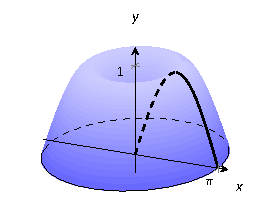
\includegraphics{figures/figshell4b}
\caption{Graphing a region in Example~\ref{eg:6.2.4}.} \label{F:6.2.Ex4b}
\end{marginfigure} % EXAMPLE

%--------------------------------------------
% SUMMARY
%--------------------------------------------
\begin{summary}
  \item We can use a definite integral to find the volume of a three-dimensional solid of revolution that results from revolving a two-dimensional region about a particular axis by taking  slices parallel to the axis of revolution which will then be cylindrical shells.
  \item If we revolve about a vertical line and slice perpendicular to that line, then our shells are vertical and of thickness $\triangle x$. This leads us to integrate with respect to $x$.
	\item If we revolve about a horizontal line and slice parallel to that line, then our shells are horizontal and of thickness $\triangle y$. This leads us to integrate with respect to $y$, as opposed to with respect to $x$ when we slice a solid vertically.
	\item Let a region $R$ be given with $x$-bounds $x=a$ and $x=b$ and $y$-bounds $y=c$ and $y=d$.
\vskip 5pt
\begin{tabular}{cccc}
 		& Washer Method & & Shell Method \rule[-10pt]{0pt}{10pt} \\
 \parbox{50pt}{\centering Horizontal Axis}  & $\ds \pi\int_a^b \big(R(x)^2-r(x)^2\big)\ dx$ & & $\ds 2\pi\int_c^d r(y)h(y)\ dy$ \\ \\
 \parbox{40pt}{\centering Vertical Axis} &  $\ds\pi \int_c^d\big(R(y)^2-r(y)^2\big)\ dy$ & & $\ds 2\pi\int_a^b r(x)h(x)\ dx$
 \end{tabular}
\index{integration!volume!Washer Method}\index{Washer Method}\index{integration!volume!Shell Method}\index{Shell Method}
\end{summary} 

\clearpage

%--------------
% EXERCISES
%--------------
\begin{adjustwidth*}{}{-2.25in}
\textbf{{\large Exercises}}
\setlength{\columnsep}{25pt}
\begin{multicols*}{2}
\noindent Terms and Concepts \small
\begin{enumerate}[1)]
\item T/F: A solid of revolution is formed by revolving a shape around an axis.
\item T/F: The Shell Method can only be used when the Washer Method fails.
\item T/F: The Shell Method works by integrating cross--sectional areas of a solid.
\item T/F: When finding the volume of a solid of revolution that was revolved around a vertical axis, the Shell Method integrates
with respect to $x$.
\end{enumerate} 

\noindent {\normalsize Problems} \small

\noindent{\bf In Exercises 5--8, a region of the Cartesian plane is shaded. Use the Shell Method to find the volume of the solid of revolution formed by revolving the region about the $y$-axis.}

\begin{enumerate}[1),resume]
\item \begin{minipage}{\linewidth}\centering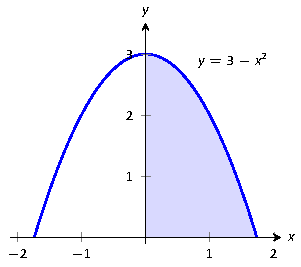
\includegraphics{figures/fig07_02_ex_09}\end{minipage}
\item \begin{minipage}{\linewidth}\centering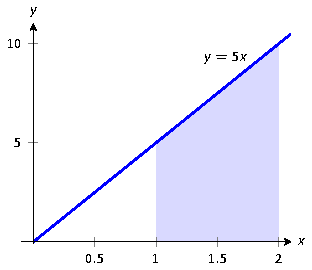
\includegraphics{figures/fig07_02_ex_06}\end{minipage}
\item \begin{minipage}{\linewidth}\centering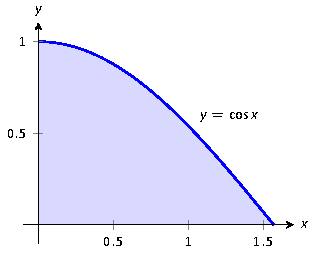
\includegraphics{figures/fig07_02_ex_07}\end{minipage}
\item \begin{minipage}{\linewidth}\centering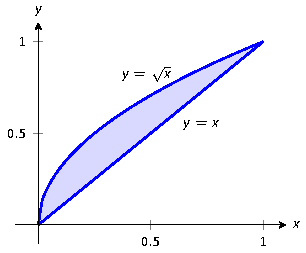
\includegraphics{figures/fig07_02_ex_04}\end{minipage}

%\item \begin{minipage}{\linewidth}\centering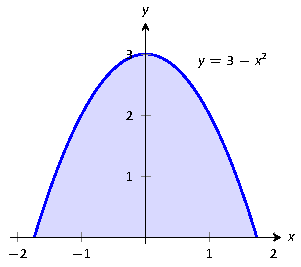
\includegraphics{figures/fig07_02_ex_05}\end{minipage}
\end{enumerate}

\noindent{\bf In Exercises 9--12, a region of the Cartesian plane is shaded. Use the Shell Method to find the volume of the solid of revolution formed by revolving the region about the $x$-axis.}

\begin{enumerate}[1),resume]
\item \begin{minipage}{\linewidth}\centering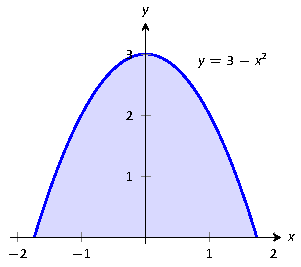
\includegraphics{figures/fig07_02_ex_05}\end{minipage}
\item \begin{minipage}{\linewidth}\centering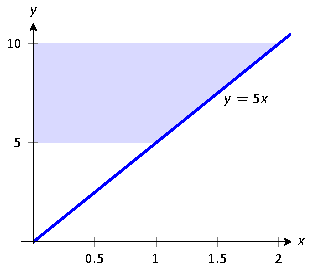
\includegraphics{figures/fig07_02_ex_10}\end{minipage}
\item \begin{minipage}{\linewidth}\centering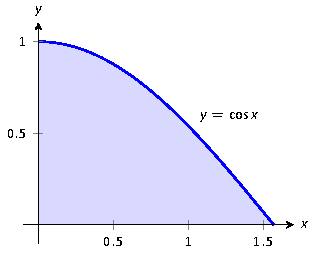
\includegraphics{figures/fig07_02_ex_07}\end{minipage}
\end{enumerate}

%------------------------------------------
% END OF EXERCISES ON FIRST PAGE
%------------------------------------------
\end{multicols*}
\end{adjustwidth*}

\clearpage

\begin{adjustwidth*}{}{-2.25in}
\setlength{\columnsep}{25pt}
\begin{multicols*}{2}\small

\begin{enumerate}[1),start=12]
\item \begin{minipage}{\linewidth}\centering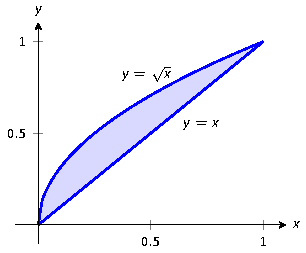
\includegraphics{figures/fig07_02_ex_04}\end{minipage}
\end{enumerate}

\vspace{.25cm}

\noindent{\bf In Exercises 13--18, a region of the Cartesian plane is described. Use the Shell Method to find the volume of the solid of revolution formed by rotating the region about each of the given axes.}

\begin{enumerate}[1),resume]
\item Region bounded by: $y=\sqrt{x}$, $y=0$ and $x=1$.

Rotate about:

\noindent%
\begin{minipage}[t]{.5\linewidth}
\begin{enumerate}
\item		the $y$-axis
\item		$x=1$
\end{enumerate}
\end{minipage}
\begin{minipage}[t]{.5\linewidth}
\begin{enumerate}\addtocounter{enumii}{2}
\item		the $x$-axis
\item		$y=1$
\end{enumerate}
\end{minipage}

\item Region bounded by: $y=4-x^2$ and $y=0$.

Rotate about:

\noindent%
\begin{minipage}[t]{.5\linewidth}
\begin{enumerate}
\item		$x=2$
\item		$x=-2$
\end{enumerate}
\end{minipage}
\begin{minipage}[t]{.5\linewidth}
\begin{enumerate}\addtocounter{enumii}{2}
\item		the $x$-axis
\item		$y=4$
\end{enumerate}
\end{minipage}

\item The triangle with vertices $(1,1)$, $(1,2)$ and $(2,1)$.

Rotate about:

\noindent%
\begin{minipage}[t]{.5\linewidth}
\begin{enumerate}
\item		the $y$-axis
\item		$x=1$
\end{enumerate}
\end{minipage}
\begin{minipage}[t]{.5\linewidth}
\begin{enumerate}\addtocounter{enumii}{2}
\item		the $x$-axis
\item		$y=2$
\end{enumerate}
\end{minipage}

\item Region bounded by $y=x^2-2x+2$ and $y=2x-1$.

Rotate about:

\noindent%
\begin{minipage}[t]{.5\linewidth}
\begin{enumerate}
\item		the $y$-axis
\item		$x=1$
\end{enumerate}
\end{minipage}
\begin{minipage}[t]{.5\linewidth}
\begin{enumerate}\addtocounter{enumii}{2}
%\item		the $y$-axis
\item		$x=-1$
\end{enumerate}
\end{minipage}

\item Region bounded by $y=1/\sqrt{x^2+1}$, $x=-1$, $x=1$ and the $x$-axis.

Rotate about:

\noindent%
\begin{minipage}[t]{.5\linewidth}
\begin{enumerate}
\item		the $y$-axis
\item		$x=1$
\end{enumerate}
\end{minipage}
\begin{minipage}[t]{.5\linewidth}
\begin{enumerate}\addtocounter{enumii}{2}
%\item		the $y$-axis
\item		$y=-1$
\end{enumerate}
\end{minipage}

\item Region bounded by $y=2x$, $y=x$ and $x=2$.

Rotate about:

\noindent%
\begin{minipage}[t]{.5\linewidth}
\begin{enumerate}
\item		the $y$-axis
\item		$x=2$
\end{enumerate}
\end{minipage}
\begin{minipage}[t]{.5\linewidth}
\begin{enumerate}\addtocounter{enumii}{2}
\item		the $x$-axis
\item		$y=4$
\end{enumerate}
\end{minipage}

\end{enumerate}

%---------------------------------------------
% END OF EXERCISES ON SECOND PAGE
%---------------------------------------------
\end{multicols*}
\end{adjustwidth*}

\afterexercises 

\cleardoublepage